\documentclass[aspectratio=169, 12pt, mathserif]{beamer}

\usepackage{fontspec}
%\usepackage{microtype}     % microtype works only with pdflatex
\usepackage[ngerman]{babel} % polyglossia makes problems with beamer

%
% temporaray packages
%
\usepackage{blindtext}

\newfontfamily\museo{Museo Slab}
\newfontfamily\helvetica{Helvetica Neue 45 Light}   % Helvetica Sans makes problems as .ttf
\setbeamerfont{frametitle}{family=\museo}
\setbeamerfont{block title}{family=\museo}
\setbeamerfont{block body}{family=\helvetica}
\setbeamerfont{title}{family=\museo}
%
% color themes and styles
%
%\usetheme{Frankfurt}
\newcommand{\thesisTitle}{Generierung und Design einer Client-Bibliothek für einen RESTful Web Service am Beispiel der Spreadshirt-API}
\newcommand{\thesisUniversityDepartment}{Fakultät für Informatik, Mathematik \& Naturwissenschaften}
\newcommand{\thesisKeyword}{Codegeneration, \textsc{Rest}ful Web Service, Modeling, Client-Library, Spreadshirt-\textsc{Api}, Polyglot}

\title[Generierung einer Client-Bibliothek aus einer WebService Beschr.]{\thesisTitle{}}
\subtitle{Bachelorverteidigung}

\author[A. Linz]{Andreas Linz}
\institute[]{\thesisUniversity{} - \thesisUniversityDepartment}

\date{\today}

\subject{Informatik}
\keywords{\thesisKeywords{}}

\begin{document}
    \begin{frame}[plain]
        \titlepage
    \end{frame} 
    
    \section*{Inhaltsverzeichnis}
    \begin{frame}{Inhaltsverzeichnis}
        \begin{multicols}{2}
            \tableofcontents
        \end{multicols}
    \end{frame}

    % introduction
    \section{Einleitung}

\subsection{Aufgabe}
\begin{frame}{Aufgabe}
    \begin{block}{Was?}
        Client-Bibliothek aus abstrakter Beschreibung eines RESTful Web Service erzeugen.
    \end{block}

    \begin{block}{Warum?}
        \begin{itemize}
            \item Vereinheitlichung bestehender Implementierungen
            \item Nutzung der API für externe Entwickler erleichtern\\(z.B. Authentifizierung kapseln)
        \end{itemize}
    \end{block}
\end{frame}

\subsection{Anforderungen}
\begin{frame}{Anforderungen}
    \begin{itemize}
        \item Austauschbarkeit der Zielsprache
        \item einfache Bedienbarkeit der Bibliothek
        \item gute Lesbarkeit des erzeugten Codes
        \item größtmögliche Typsicherheit des erzeugten Codes
        \item {\color{gray} hohe Testabdeckung}
        \item vollständige Generierung der Methoden aus der API-Beschreibung
    \end{itemize}
\end{frame}

\subsection{Spreadshirt}
\begin{frame}{Spreadshirt}
    \begin{itemize}
        \item führendes Unternehmen für \emph{personalisierte Bekleidung}
        \item \emph{Social-Commerce} (Interaktion mit Kunden steht im Vordergrund) %subset of eCommerce
        \item Standorte in Europa \& Nordamerika, HQ in Leipzig
        \item $\approx$ 450 Mitarbeiter, 50 in der IT
        \item $4*10^5$ Spreadshirt-Shops mit $33*10^6$ Produkten
    \end{itemize}
\end{frame}

\subsection{Spreadshirt-API}
\begin{frame}[squeeze]
    \begin{itemize}
        \item Online-Plattform um Kleidungsstücke, Accessoires und mehr selbst zu:
        \begin{itemize}
            \item gestalten
            \item kaufen
            \item zum Verkauf anbieten (eigene Designs als Motiv oder Produkt)
        \end{itemize}
    \end{itemize}

    \begin{block}{Spreadshirt-API}
        \begin{itemize}
            \item API erlaubt Entwicklern die Nutzung eines großen Teils der Funktionen der Online-Plattform in eigenen Applikationen
            \item u.a. Produkterstellung, Designupload \& Warenkorbverwaltung
            \item Erstellen eigener Shops und kundenspezifischer Anwendungen %( personalisierte Werbung )
        \end{itemize}
    \end{block}
\end{frame}

\begin{frame}
    \begin{figure}
        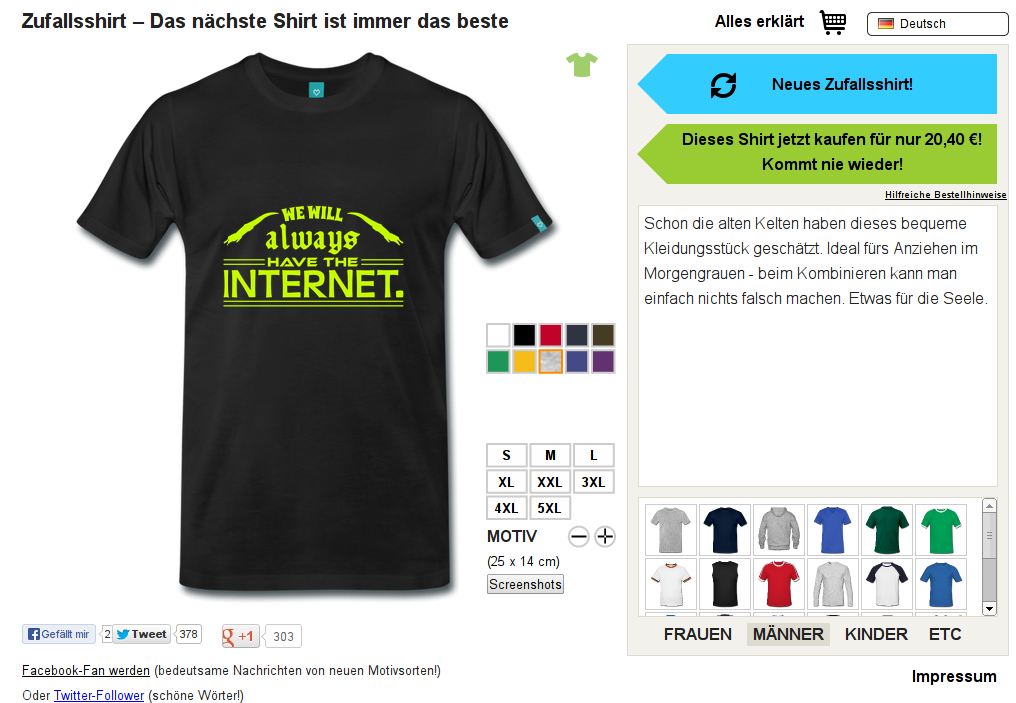
\includegraphics[height=0.8\textheight]{resources/zufallsshirt}
        \caption{Beispiel für kundenspezifische Anwendung: zufallsshirt.de}
    \end{figure}
\end{frame}


    % mainpart
    \section{Hauptteil}

\subsection{Web Services}
\begin{frame}{RESTful Web Service}
    \begin{block}{REST}
        \begin{itemize}
            \item \emph{Representational State Transfer} (Gegenständlicher Zustandstransfer)
            \item Softwarearchitekturstil für Webanwendungen
            \item Anwendungen bestehen aus \emph{Ressourcen} mit eindeutigem Bezeichner (\cref{restURI}) %(alles was sich über Bezeichner referenzieren lässt, z.B. Dokumente, Dienste oder Sammlungen von Diensten)
            \item Zustand einer Ressource ist eine \emph{Repräsentation}
            \item Aktionen mit einer REST-API über den Austausch von Repräsentationen
        \end{itemize}
    \end{block}
\end{frame}

\begin{frame}
    \begin{figure}
        \centering
        \[
            \underbrace{\texttt{http://api.spreadshirt.net/api/v1/}}_{Basis-URL}\underbrace{\overbrace{\texttt{baskets/84}}^{Warenkorb}\overbrace{\texttt{/item/42}}^{Artikel}}_{Ressource}
        \]
        \caption{Beispiel-URI, um den Artikel 42 aus dem Warenkorb 84 anzusprechen}
        \label{restURI}
    \end{figure}
    \emph{RESTful Web Service} ist eine Webanwendung die den REST Prinzipien entspricht
\end{frame}

\subsection{Dokumentbeschreibungssprachen}
\begin{frame}[squeeze]{Dokumentbeschreibungssprachen}
    \begin{block}{WADL}
        maschinenlesbare Beschreibung einer HTTP-basierten Webanwendung
    \end{block}
    \begin{block}{XSD}
        Dokumentbeschreibungssprache zur Definition von Datentypen
    \end{block}
    Gemeinsamkeiten:
    \begin{itemize}
        \item XML-Syntax, selbst wieder gültige XML-Dokumente
        \item Baumgrammatiken
    \end{itemize}
\end{frame}

\subsection{Codegenerierung}
\begin{frame}{Codegenerierung}

    \begin{block}{Codegenerator}
        Programm welches aus einer \emph{höhersprachigen Spezifikation}, einer Software oder eines Teilaspektes, die \emph{Implementierung erzeugt}
    \end{block}
    \begin{block}{Vorteile}
        \begin{itemize}
            \item Produktivitässteigerung
            \item hohe Konsistenz des Generats
            \item zentrale Stelle für Änderungen (Eingabemodell)
        \end{itemize}
    \end{block}
\end{frame}

\begin{frame}{Generatorformen}
    \begin{block}{Klassifikation nach Generierungsmenge}
        \begin{itemize}
            \item teilweise
            \begin{itemize}
                \item Inline-Code Expander
                \item Mixed-Code Generator
                \item Partial-Class Generator
            \end{itemize}
            \item vollständig (Tier\footnote{Stufen}-Generator)
            \item mehrfach (n-Tier Generator)
        \end{itemize}
    \end{block}
\end{frame}

\subsection{Datenmodelle \& Codegenerator}
\begin{frame}{Datenmodelle}
    Eingabe des Generators
    \begin{itemize}
        \item Applikationsmodell:
        \begin{itemize}
            \item WADL $\rightarrow{}$ REST-Modell
            \item XSD $\rightarrow{}$ Schema-Modell
        \end{itemize}
        \item Sprachenmodell
        \begin{itemize}
            \item kapselt Zielsprache
            \item enthält Semantik
            \item[!] Syntax in Ausgabemodul (LanguageVisitor, siehe \cref{sequence})
        \end{itemize}
    \end{itemize}
\end{frame}

\begin{frame}{Generator für die Spreadshirt-API}
    \begin{figure}
        \resizebox{\textwidth}{!}{
            \begin{tikzpicture}[
        node distance=12mm and 8mm,
        every node/.style={font=\scriptsize}
    ]
    % Blocks
    \node(abstractDescription)[greyBlock]{Abstrakte\\Beschreibung\\der Spreadshirt-API};
    \node(dummy1)[dummy, right=of abstractDescription]{};
    \node(wadlAnalysis)[greyBlock, above=of abstractDescription]{Analyse\\WADL-Datei};
    \node(restModel)[greyBlock, right=of wadlAnalysis]{REST-\\Modell};
    \node(xsdAnalysis)[greyBlock, below=of abstractDescription]{Analyse\\XSD-Datei};
    \node(schemaModel)[greyBlock, right=of xsdAnalysis]{Schema-\\Modell};
    \node(modelCombine)[greyBlock, right=of dummy1]{Kombinierer};
    \node(applicationModel)[greyBlock, right=of modelCombine]{Applikations-\\Modell};
    \node(generator)[greyBlock, right=of applicationModel]{Generator};
    \node(languageModel)[greyBlock, right=of generator]{Zielsprachen-\\Modell};
    \node(languageFactory)[greyBlock, below=of generator]{Language-\\Factory};
    \node(filePrinter)[greyBlock, right=of languageModel]{Ausgabemodul\\(File Printer)};
    \node(languageVisitor)[greyBlock, above=of filePrinter]{Language-\\Visitor};
    \node(library)[greyBlock, double copy shadow, right=of filePrinter]{Bibliotheks-\\Dateien};
    \node(staticFiles)[greyBlock, double copy shadow, below=of library]{Statische Dateien};

    %\node(languagemodel)[greyBlock, right= of generator]{Sprachenmodell\\\emph{Abstrakter Syntaxbaum}};
    % Lines  
    \path[arrow, ->] (abstractDescription) -- (wadlAnalysis);
    \path[arrow, ->] (abstractDescription) -- (xsdAnalysis);
    \path[arrow, ->] (wadlAnalysis) -- (restModel);
    \path[arrow, ->] (xsdAnalysis) -- (schemaModel);
    \path[arrow, ->] (restModel) -- (modelCombine);
    \path[arrow, ->] (schemaModel) -- (modelCombine);
    \path[arrow, ->] (modelCombine) -- (applicationModel);
    \path[arrow, ->] (applicationModel) -- (generator);
    \path[arrow, ->] (languageFactory) -- (generator);
    \path[arrow, ->] (generator) -- (languageModel);
    \path[arrow, ->] (languageModel) -- (filePrinter);
    \path[arrow, ->] (languageVisitor) -- (filePrinter);
    \path[arrow, ->] (filePrinter) -- (library);
    \path[arrow, ->] (staticFiles) -- (library);

    %\path[arrow, ->] (infrastructurecode) -- (generator);
\end{tikzpicture}

        }
        \caption{Sequenzdiagramm des Generators für die Spreadshirt-API}
        \label{sequence}
    \end{figure}
\end{frame}

\subsection{Client-Bibliothek}
\begin{frame}{Datenklassen}
    \begin{itemize}
        \item zielsprachenabhängige Repräsentation der Typen aus der XML-Schema Beschreibung
        \item Variablen bilden die Attribute und Elemente aus dem Schematyp ab
        \item Getter- und Setter-Methoden für alle Variablen
        \item transportunabhäniger Datenaustausch mit API $\rightarrow{}$ Methoden zur Serialisierung und Deserialisierung
    \end{itemize}
\end{frame}

\begin{frame}[fragile,squeeze]
    \begin{multicols}{2}
        \begin{lstlisting}[
                %caption=Point-Klasse als (gekürztes) Beispiel für eine generierte Datenklasse,
                language=PHP
            ]
<?php
   require_once('Unit.php');

   class Point
   {
      private $unit; // unit 
      private $y; // double 
      private $x; // double 

      function __construct(
            /* double */ $y,
            /* double */ $x
         )
      {
         $this->y = $y;
         $this->x = $x;
      }

      public function setUnit(
            /* unit */ $unit
         )
      {
         $this->unit = $unit;
      }
      ...
      public function toXML()
      {
         $xml =  new SimpleXMLElement(/* Point */ '<login xmlns="http://api.spreadshirt.net"/>');
         $xml->addChild(/* string */ 'unit',/* unit */ $this->unit);
         $xml->addChild(/* string */ 'y',/* double */ $this->y);
         $xml->addChild(/* string */ 'x',/* double */ $this->x);
         return $xml->asXML();
      }
      ...
      public function getX()
      {
         return $x = $this->x;
      }
   }
?>
        \end{lstlisting}
    \end{multicols}
\end{frame}

\begin{frame}{Ressourcenklassen}
    \begin{itemize}
        \item zielsprachenabhängige Abbildung der Ressourcenbeschreibungen aus WADL-Datei
        \item Methoden der Klassen entsprechen den Methoden der abgebildeten Ressource
    \end{itemize}
\end{frame}

\begin{frame}[fragile, squeeze]
    \begin{lstlisting}[
        %caption=Klasse zur Ressource \texttt{users/{userId}/products} als Beispiel für eine Ressourcenklasse,
        language=PHP
    ]
<?php
   require_once('Static/methods.php');
   require_once('Static/apiUser.php');
   /* Create or list products for user. */
   class UsersUserIdProducts
   {
      private $baseUrl = 'http://192.168.13.10:8080/api/v1/'; // string
      ...
      /*  */
      public function POST(
            /* array */ $parameters, 
            /* ApiUser */ $apiUser,
            /* ProductDTO */ $productDTO
         )
      { ... }
      ...
      function __construct(
            /* string */ $userId
         )
      {
         $this->userId = $userId;
         $this->resourceUrl = $this->baseUrl . 'users' . '/' . $userId . 'products';
      }
   }
?>
    \end{lstlisting}
\end{frame}

\begin{frame}{statische Klassen}
    \begin{itemize}
        \item wurden manuell erstellt
        \item enthalten gemeinsam genutzten Code ohne variable Bestandteile
        \item Bibliothek enthält zwei dieser Klassen:
        \begin{itemize}
            \item Kommunikation über HTTP-Methoden mit der API
            \item Kapselung der Authentifizierung
        \end{itemize}
    \end{itemize}
\end{frame}

    % end
    \section{Zusammenfassung}

\begin{frame}{Zusammenfassung}
    \begin{itemize}
        \item Entwicklung der Datenmodelle
        \item Überführung der Beschreibung in Eingabedatenmodelle des Generators
        \item Erstellung und Implementierung des Sprachenmodells für PHP
        \item Implementierung des Generators
        \item Generierung der Bibliothek
    \end{itemize}
\end{frame}

\subsection{Ausblick}
\begin{frame}{Ausblick}
    \begin{itemize}
        \item Parameterobjekte
        \item {\color{gray} Fluent-Interface}
        \item Java-Bibliothek (Sprachenmodell)
        \item Erzeugung von Dokumentation und Testdaten
    \end{itemize}
\end{frame}

\subsection{Diskussion}
\begin{frame}{Diskussion}
    \begin{itemize}
        \item XSD, WADL
        \item RESTful Web Services
        \item Datenmodelle für Web Service Beschreibung und Programmiersprache
        \item Stufen-Generator
        \item PHP Client-Bibliothek
    \end{itemize}
\end{frame}
\end{document}
